\documentclass{article}
\usepackage[utf8]{inputenc}
\usepackage[spanish]{babel}
\usepackage{listings}
\usepackage{graphicx}
\graphicspath{ {images/} }
\usepackage{cite}

\begin{document}

\begin{titlepage}
    \begin{center}
        \vspace*{1cm}
            
        \Huge
        \textbf{Parcial 1 - Calistenia.}
            
        \vspace{0.5cm}
        \LARGE
            
        \vspace{1.5cm}
            
        \textbf{Luis Miguel Gil Rodriguez.}
            
        \vfill
            
        \vspace{0.8cm}
            
        \Large
        Despartamento de Ingeniería Electrónica y Telecomunicaciones\\
        Universidad de Antioquia\\
        Medellín\\
        Marzo de 2021
            
    \end{center}
\end{titlepage}

\tableofcontents
\newpage
\section{Sección introductoria.}\label{intro}
En este documento, podremos encontrar las instrucciones para llevar unos objetos desde una posicion A, hasta una posición B, intentando ser lo mas detallado posible.
\\
\\
En la figura (\ref{fig:pos_a}), se presenta la posición inicial del experimento, donde las dos tarjetas estan debajo de la hoja de papel.
\begin{figure}[h]

\includegraphics[width=5cm]{pos_a.jpg}
\centering
\caption{Posición A.}
\label{fig:pos_a}
\end{figure}
\\
En la Figura (\ref{fig:pos_b}), se presenta la posiicon final del experimento, donde las dos tarjetas estan sobre la hoja de papel formando una especie de piramide de naipes.
\begin{figure}[h]
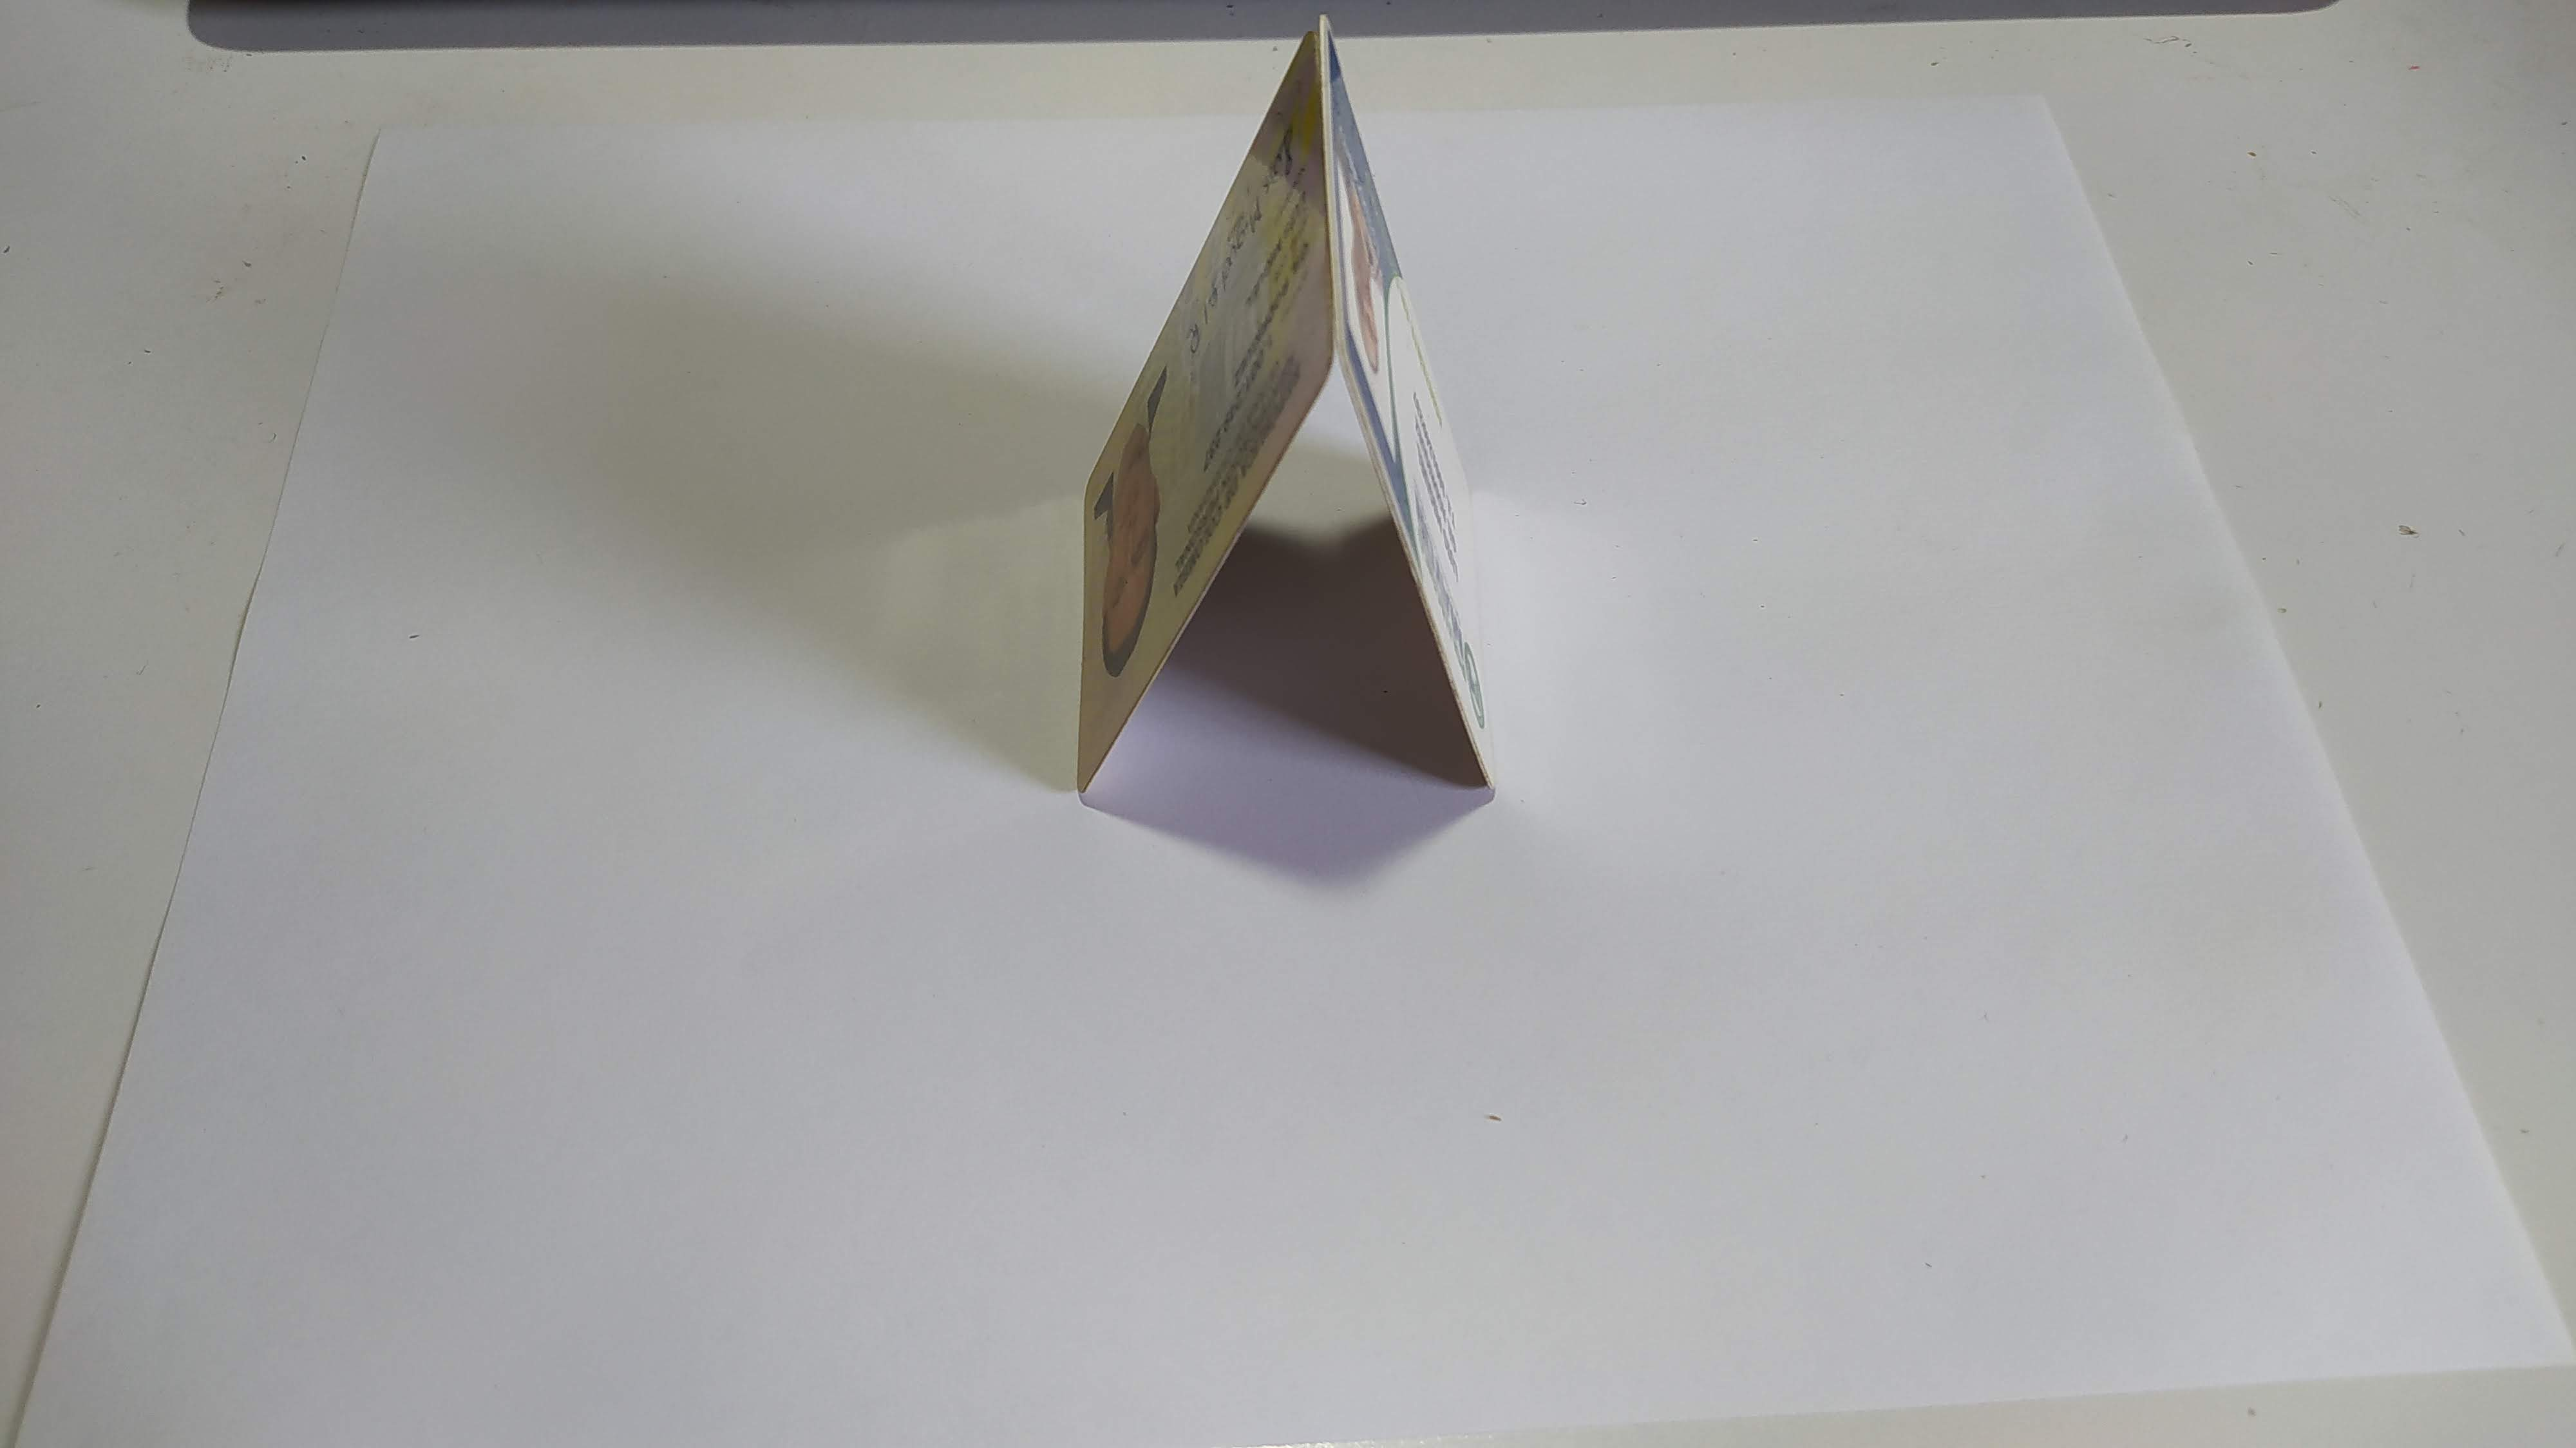
\includegraphics[width=5cm]{pos_b.jpg}
\centering
\caption{Posición B.}
\label{fig:pos_b}
\end{figure}

\section{Intrucciones a seguir.} \label{contenido}
\textbf{Para tener en cuenta:}  Para el siguiente experimento solo debe utilizar su mano dominante. En ningún momento del experimento puedo agarrar los elementos con sus dos manos.
\begin{enumerate}
  \item Mover la hoja de papel a un punto cualquiera de la mesa, de modo que las tarjetas que hay debajo de la hoja queden completamente descubiertas.
  \item Poner las tarjetas juntas en otra parte de la mesa (forma horizontal). Nota: No se pueden poner encima de la hoja y aproximadamente a unos 20 centímetros de su posición inicial.
  \item Retorne la hoja de papel a su posición inicial. (forma horizontal).
  \item Levante las dos tarjetas unos 20 centímetros sin separarlas, de sus contornos más largos haciendo uso de todos los dedos de la mano y manténgalas levantadas, pues es requisito para el siguiente paso.
  \item Si su mano dominante es la Derecha, girar las tarjetas 90 grados en dirección de las manecillas de reloj de modo que usted no puede ver ninguna de las caras de ambas tarjetas cuando las coloque enfrente suyo y que las tarjetas estén en posición vertical. De lo contrario, girar las tarjetas 90 grados en dirección contraria de las manecillas del reloj de modo que usted no puede ver ninguna de las caras de ambas tarjetas cuando las coloque enfrente suyo y que las tarjetas estén en posición vertical.
  \item Apoye las dos tarjetas en el centro de la hoja de modo que entre las tarjetas y la hoja exista un ángulo de 90 grados.
  \item Si su mano dominante es la derecha deslice la tarjeta que se encuentra en el lado derecho suavemente hasta formar una especie de pirámide naipes y que esta esté en equilibrio. De lo contrario, haga lo mismo con la tarjeta que se encuentra del lado izquierdo.
  \item Si no logro poner las tarjetas en equilibrio, repita los pasos del 4 al 7, de lo contrario, Felicitaciones, finalizaste el experimento.
\end{enumerate}
\cite{list_latex}
\section{Link del video.} \label{Link del video}
Link: https://youtu.be/jNcfbtZos8k

\section{Conclusiones.} \label{imagenes}
Es probable que muchas personas no logren ver la importancia de este experimento, pero ese no mi caso; hablando desde el ámbito de la programación, esta sencilla prueba es una ayuda para comprender que tan fundamental es la buena codificación de un programa, siendo lo menos ambiguo posible, sin caer en redundancias o peor aun en contradicciones. Todo esto será de útil ayuda para lograr un bien nivel de lógica de programación, entender y codificar de una manera más eficiente.
\\
\\
Ahora bien, fuera del ámbito de la programación, este experimento también cobra importancia, no nos alejemos tanto de nuestra situación y pensemos ¿qué sería de un profesor que no se supiera como explicar bien los temas?, es muy probable que la gran mayoría de sus estudiantes terminen cancelando el curso. Ahora, pensemos a futuro, ¿qué sería de un jefe que no sepa cómo dar instrucciones precisas y concisas?, es muy probable que todo el proyecto que en el que se encuentran trabajando salga mal o bien tarde más tiempo de lo esperado. Por lo que una correcta comunicación e impartición de instrucciones es fundamental para poder llevar a cabo un proyecto en grupo.

\bibliographystyle{IEEEtran}
\bibliography{references}
\end{document}
